\documentclass[a4paper]{scrartcl}
\usepackage{scrpage2}
\usepackage[ngerman]{babel}
\usepackage[T1]{fontenc}
\usepackage[utf8]{inputenc}
%\usepackage[pdftex]{graphicx}
%\usepackage[intlimits]{amsmath}
%\usepackage{listings}
%\lstset{frame=single,breaklines=true}
\usepackage{ amssymb }
\usepackage{amsmath}
\usepackage{hyperref}
\usepackage{enumerate}
\usepackage[a4paper, total={19cm, 23cm}]{geometry}
\usepackage{stmaryrd}
\usepackage{esvect}
\usepackage{graphicx}
\pagestyle{scrheadings}
\pagenumbering{gobble}
\ihead{Übungsblatt 6\\Nils Werner 108012219293}
\chead{\\Paul Rösler 108012225686	}
\ohead{Übungsgruppe: Mo. 16:00\\(Daniel Teuchert 108012214552)}
\setheadsepline{0.4pt}
\begin{document}

\section*{Aufgabe 1}
\begin{enumerate}[a)]
\item $ \langle \alpha  | \beta \rangle  = \frac{1}{\sqrt{N-M}} \frac{1}{\sqrt{M}} \sum_{f(x')=0} \langle x' | \sum_{f(x)=1} | x \rangle$\\
$=\frac{1}{\sqrt{N-M} \sqrt{M}} \sum_{x'\neq x} \langle x' | x \rangle = 0$\\
$\Rightarrow |\alpha \rangle$ und $| \beta \rangle$ sind orthogonal.

\item $ | \psi \rangle = \frac{1}{\sqrt{N}} \sum_y |y\rangle = \frac{1}{\sqrt{N}} (\sum_{y: f(y) = 0} |y\rangle + \sum_{y: f(y) = 1} |y\rangle)$\\
$= \frac{1}{\sqrt{N}} \sum_{f(x') = 0} |x'\rangle + \frac{1}{\sqrt{N}} \sum_{f(x) = 1} |x\rangle$\\
$= \frac{1}{\sqrt{N}} \frac{\sqrt{N-M}}{\sqrt{N-M}} \sum_{f(x') = 0} |x'\rangle + \frac{1}{\sqrt{N}} \frac{\sqrt{M}}{\sqrt{M}} \sum_{f(x) = 1} |x\rangle$\\
$= \frac{\sqrt{N-M}}{\sqrt{N}} (\frac{1}{\sqrt{N-M}} \sum_{f(x') = 0} |x'\rangle) + \frac{\sqrt{M}}{\sqrt{N}} (\frac{1}{\sqrt{M}} \sum_{f(x) = 1} |x\rangle)$\\
$= \frac{\sqrt{N-M}}{\sqrt{N}} |\alpha \rangle + \frac{\sqrt{M}}{\sqrt{N}} |\beta \rangle = c_{\alpha} |\alpha \rangle + c_{\beta} |\beta \rangle$\\

\item $WV | \gamma^{(i-1)} \rangle = (-I_n +2 |\psi \rangle \langle \psi | ) ~ (I_n - 2 |\bar{a} \rangle \langle \bar{a}| ) ~ | \gamma^{(i-1)} \rangle$ mit $|\bar{a} \rangle = |\beta \rangle$\\
$= (-I_n +2 (c_{\alpha} |\alpha \rangle + c_{\beta} |\beta \rangle) (c_{\alpha} \langle \alpha| + c_{\beta} \langle \beta|) ) ~ (I_n - 2 | \beta \rangle \langle \beta| ) ~ | \gamma^{(i-1)} \rangle$\\
$= (-I_n +2 c_{\alpha}^2 |\alpha \rangle \langle \alpha| + 2 c_{\alpha} c_{\beta} ( |\alpha \rangle \langle \beta| + |\beta \rangle \langle \alpha|) + 2 c_{\beta}^2 |\beta \rangle \langle \beta| ) ~ (I_n - 2 | \beta \rangle \langle \beta| ) ~ | \gamma^{(i-1)} \rangle$\\
$= (-I_n +2 c_{\alpha}^2 |\alpha \rangle \langle \alpha| + 2c_{\alpha}c_{\beta} ( |\alpha \rangle \langle \beta| + |\beta \rangle \langle \alpha|) + 2c_{\beta}^2 |\beta \rangle \langle \beta| + 2 | \beta \rangle \langle \beta| - 4 c_{\alpha}c_{\beta} |\alpha \rangle \langle \beta| - 4 c_{\beta}^2 |\beta \rangle \langle \beta| ) ~ | \gamma^{(i-1)} \rangle$\\
$= 2(- \frac{1}{2}I_n + c_{\alpha}^2 |\alpha \rangle \langle \alpha| - c_{\alpha}c_{\beta} |\alpha \rangle \langle \beta| + c_{\alpha}c_{\beta} |\beta \rangle \langle \alpha| + (1 - c_{\beta}^2) |\beta \rangle \langle \beta|) ~ (c_{\alpha}^{(i-1)} |\alpha \rangle + c_{\beta}^{(i-1)} |\beta \rangle)$\\
$= (-c_{\alpha}^{(i-1)} + 2c_{\alpha}^2 c_{\alpha}^{(i-1)} - 2c_{\alpha}c_{\beta} c_{\beta}^{(i-1)}) |\alpha \rangle + (-c_{\beta}^{(i-1)} + 2c_{\alpha}c_{\beta} c_{\alpha}^{(i-1)} + 2(1 - c_{\beta}^2) c_{\beta}^{(i-1)} ) |\beta \rangle = | \gamma^{(i)} \rangle$\\

$\Rightarrow  \begin{pmatrix} c_{\alpha}^{(i)}\\ c_{\beta}^{(i)}\end{pmatrix} = G \begin{pmatrix} c_{\alpha}^{(i-1)}\\ c_{\beta}^{(i-1)}\end{pmatrix} \stackrel{!}{=} \begin{pmatrix}-c_{\alpha}^{(i-1)} + 2c_{\alpha}^2 c_{\alpha}^{(i-1)} - 2c_{\alpha}c_{\beta} c_{\beta}^{(i-1)} \\ -c_{\beta}^{(i-1)} + 2c_{\alpha}c_{\beta} c_{\alpha}^{(i-1)} + 2(1 - c_{\beta}^2) c_{\beta}^{(i-1)} \end{pmatrix}$\\

$\begin{pmatrix} cos \theta & -sin \theta\\ sin \theta & cos \theta \end{pmatrix} \begin{pmatrix} c_{\alpha}^{(i-1)}\\ c_{\beta}^{(i-1)}\end{pmatrix}$\\
$= \begin{pmatrix} 2 cos^2 \frac{\theta}{2}-1 & -2 sin \frac{\theta}{2} cos \frac{\theta}{2} \theta\\ 2 sin \frac{\theta}{2} cos \frac{\theta}{2} & 2 cos^2 \frac{\theta}{2}-1 \end{pmatrix} \begin{pmatrix} c_{\alpha}^{(i-1)}\\ c_{\beta}^{(i-1)}\end{pmatrix}$\\
$= \begin{pmatrix} 2 \langle \alpha | \psi \rangle^2 -1 & -2 \langle \beta | \psi \rangle \langle \alpha | \psi \rangle \\ 2 \langle \beta | \psi \rangle \langle \alpha | \psi \rangle & 2 \langle \alpha | \psi \rangle^2 -1 \end{pmatrix} \begin{pmatrix} c_{\alpha}^{(i-1)}\\ c_{\beta}^{(i-1)}\end{pmatrix}$\\
$= \begin{pmatrix} 2 c_{\alpha}^2 -1 & -2 c_{\alpha}c_{\beta} \\ 2 c_{\alpha}c_{\beta} & 2 c_{\alpha}^2 -1 \end{pmatrix} \begin{pmatrix} c_{\alpha}^{(i-1)}\\ c_{\beta}^{(i-1)}\end{pmatrix}
= \begin{pmatrix} 2c_{\alpha}^2 c_{\alpha}^{(i-1)} -c_{\alpha}^{(i-1)} - 2c_{\alpha}c_{\beta} c_{\beta}^{(i-1)} \\ 2c_{\alpha}c_{\beta} c_{\alpha}^{(i-1)} + 2c_{\alpha}^2 c_{\beta}^{(i-1)} -c_{\beta}^{(i-1)}\end{pmatrix}$\\

Für $G_{2,2} = -(2 c_{\beta}^2 -1) = ?$ würde das Ergebnis stimmen.

\end{enumerate}


\newpage
\section*{Aufgabe 2}
\begin{enumerate}[a)]
\item
Der Schaltkreis für $W$ ergibt sich aus der Übung für die Funktion $g'(x) = \begin{cases} 1, x\neq 0\\ 0, sonst \end{cases}$.

\begin{figure}[htp] \centering{
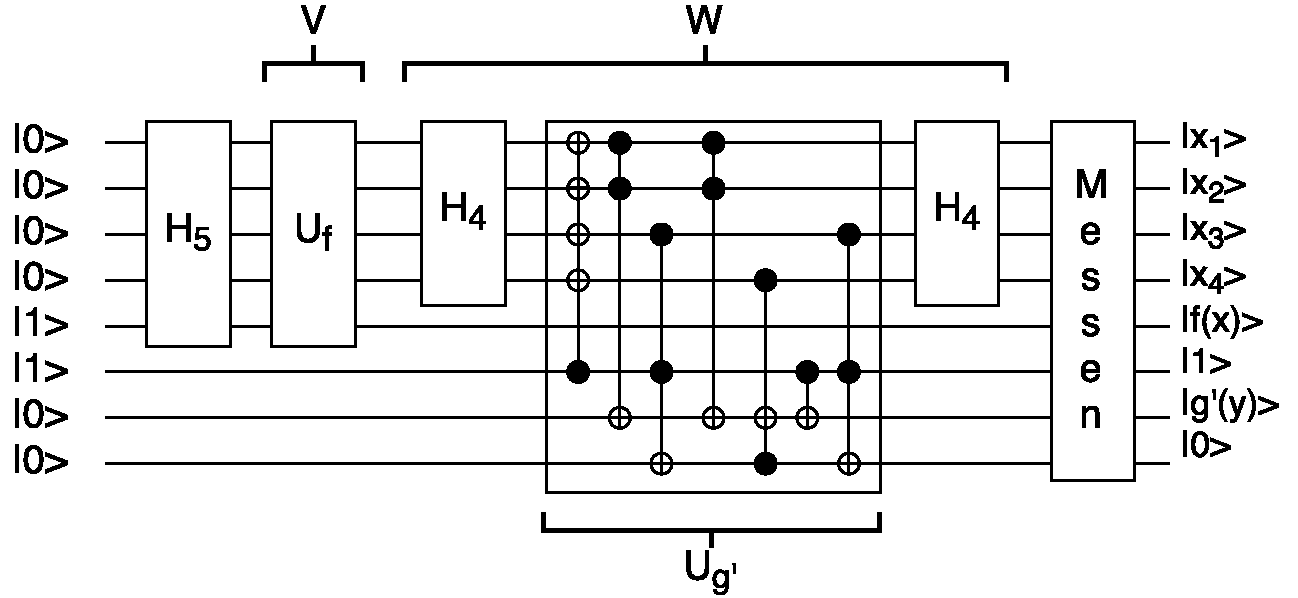
\includegraphics[scale=0.8]{grover.pdf}}
\caption{Quantenschaltkreis für eine Grover-Iteration $WV|\psi\rangle$ auf 4 Qubits für die Funktion $f$}
\end{figure}

\item $|\alpha\rangle = \frac{1}{\sqrt{16-3}} \sum_{f(x')=0} |x'\rangle,~ |\beta\rangle = \frac{1}{\sqrt{3}} \sum_{f(x)=1} |x\rangle$\\
$c_{\alpha}^{(0)} = \frac{\sqrt{13}}{\sqrt{16}},~ c_{\beta}^{(0)} = \frac{\sqrt{3}}{4}$\\

Obwohl wir in Aufgabe 1) einen Fehler gemacht haben, wird hier weiter mit der Matrix aus der Aufgabenstellung gerechnet:\\

$\begin{pmatrix} c_{\alpha}^{(1)}\\ c_{\beta}^{(1)}\end{pmatrix} = \begin{pmatrix} 2 \langle \alpha | \psi \rangle^2 -1 & -2 \langle \beta | \psi \rangle \langle \alpha | \psi \rangle \\ 2 \langle \beta | \psi \rangle \langle \alpha | \psi \rangle & 2 \langle \alpha | \psi \rangle^2 -1 \end{pmatrix} \begin{pmatrix} c_{\alpha}^{(0)}\\ c_{\beta}^{(0)}\end{pmatrix}$\\
$=\begin{pmatrix} 2 (c_{\alpha}^{(0)})^2 -1 & -2 c_{\beta}^{(0)} c_{\alpha}^{(0)} \\ 2 c_{\beta}^{(0)} c_{\alpha}^{(0)} & 2 (c_{\alpha}^{(0)})^2 -1 \end{pmatrix} \begin{pmatrix} c_{\alpha}^{(0)}\\ c_{\beta}^{(0)}\end{pmatrix}$\\
$= \begin{pmatrix} 2 (c_{\alpha}^{(0)})^3 -c_{\alpha}^{(0)} - 2c_{\alpha}^{(0)} (c_{\beta}^{(0)})^2 \\ 2(c_{\alpha}^{(0)})^2c_{\beta}^{(0)} + 2(c_{\alpha}^{(0)})^2c_{\beta}^{(0)} -c_{\beta}^{(0)}\end{pmatrix}$\\

$= \begin{pmatrix} \frac{13\sqrt{13}}{32} - \frac{\sqrt{13}}{4} - \frac{3\sqrt{13}}{32} \\ \frac{13\sqrt{3}}{16} - \frac{\sqrt{3}}{4}\end{pmatrix} = \begin{pmatrix}\frac{\sqrt{13}}{16} \\ \frac{9\sqrt{3}}{16}\end{pmatrix}$\\

$\Rightarrow |\gamma^{(1)}\rangle = c_{\alpha}^{(1)} |\alpha\rangle + c_{\beta}^{(1)} |\beta\rangle = \frac{\sqrt{13}}{16} |\alpha\rangle + \frac{9\sqrt{3}}{16} |\beta\rangle
= \frac{1}{16} \sum_{f(x')=0} |x'\rangle+ \frac{9}{16} \sum_{f(x)=1} |x\rangle$\\
$= \frac{1}{16} (\sum_{f(x')=0} |x'\rangle+ 9 \sum_{f(x)=1} |x\rangle)$\\

\item Für eine Grover-Iteration: $(\frac{9}{16})^2*3 = \frac{243}{256} \approx 0,949$

$\begin{pmatrix} c_{\alpha}^{(2)}\\ c_{\beta}^{(2)}\end{pmatrix} = \begin{pmatrix} 2 \langle \alpha | \psi \rangle^2 -1 & -2 \langle \beta | \psi \rangle \langle \alpha | \psi \rangle \\ 2 \langle \beta | \psi \rangle \langle \alpha | \psi \rangle & 2 \langle \alpha | \psi \rangle^2 -1 \end{pmatrix} \begin{pmatrix} c_{\alpha}^{(1)}\\ c_{\beta}^{(1)}\end{pmatrix}$\\
$=\begin{pmatrix} 2 (c_{\alpha}^{(0)})^2 -1 & -2 c_{\beta}^{(0)} c_{\alpha}^{(0)} \\ 2 c_{\beta}^{(0)} c_{\alpha}^{(0)} & 2 (c_{\alpha}^{(0)})^2 -1 \end{pmatrix} \begin{pmatrix} c_{\alpha}^{(1)}\\ c_{\beta}^{(1)}\end{pmatrix}$\\
$=\begin{pmatrix} \frac{13}{8}-1 & - \frac{\sqrt{3}\sqrt{13}}{8} \\ \frac{\sqrt{3}\sqrt{13}}{8} & \frac{13}{8}-1 \end{pmatrix} \begin{pmatrix}\frac{\sqrt{13}}{16} \\ \frac{9\sqrt{3}}{16}\end{pmatrix} = \begin{pmatrix} \delta \\ \frac{29\sqrt{3}}{64}\end{pmatrix}$ da $c_{\alpha}^{(2)}$ nicht wichtig, $\delta$ nicht berechnet.\\

$\Rightarrow$ Für zwei Grover-Iterationen $(\frac{29\sqrt{3}}{64} \frac{1}{\sqrt{3}})^2*3 = \frac{2523}{4069} \approx 0,616$

\end{enumerate}

\newpage
\section*{Aufgabe 3}
\begin{enumerate}[a)]
\item
\item

\end{enumerate}

\end{document}
